\section{The AMIDST requirements engineering process}
\label{sec:AmidstRequirementProcess}

This section contains a description of the AMIDST RE process.  We first describe the main characteristics of AMIDST and continue by describing the RE process in relation to these characteristics.

%Prior to project start, the importance of requirement engineering was well acknowledged by the partners in the project.  This is evident from the %fact that 23 out of 310 person months were assigned to conduct the requirement analysis.  We have chosen to summarize the characteristics in t%he next subsections, which makes it is easier to refer to them later in this report.
\subsection{Characteristics of the AMIDST project}
\label{sec:characteristics}

In this subsection, we list the main aspects or characteristics of the project that have the greatest impact on the design of the RE process.  Notice, that there are also many other characteristics of AMIDST that are not mentioned here.  This is because their impact on the RE process is believed to be minimal.  
%It is also worth noting that other researchers and practitioners that want to follow our path of describing characteristics of the project, may benefit from our analyses of which characteristics had the most impact on the RE process.


\subsubsection*{Characteristics one:  Pre-specified scope of the project}
\label{sec:characteristic1}

When the AMIDST project started, there was a document of work that was already agreed upon.  In particular the RE process must comply with this document and the software must comply with the deliveries in the work package one to eight.  In practice, this means that whenever a requirement is considered, it must always be justified and linked with a delivery in a work package.

\subsubsection*{Characteristics two: Many partners on different locations}
\label{sec:characteristic2}
The project is a consortium of 7 partners, 4 industrial and 3 universities, which are situated in 4 different countries.  The result is a project with many stakeholders, which have different backgrounds, priorities and influences on the software. Moreover, the partners are located in different countries, which implies that the financial and time costs for personal meetings are quite high.  This characteristic has an influence on the pursued RE process, because the process is restricted to not rely heavily on meetings with many participants.

\subsubsection*{Characteristics three: Transference of domain knowledge between industrial and academic partners}
\label{sec:characteristic3}

The industrial partners of the AMIDST project come from very different domains: automotive, energy and finance industry.  On one side, it was essential that the industrial partners gained enough insight of what can be done with probabilistic graphical models to identify proper use cases.  On the other side, it was essential that the academic partners gained enough knowledge about the industrial domains to understand the proposed use cases and requirements.
%This was considered in the way we divided our work among the academic partners. 

\subsubsection*{Characteristics four:  One framework for three different problems}
\label{sec:characteristic4}

The main aim of AMIDST software is to give solutions to the problems that are posed by the three industrial partners.  One single framework shall solve all posed problems.  It is therefore a challenge to find common requirements that are addressing problems across all three domains.

\subsubsection*{Characteristics five: Targets are not fully defined}
\label{sec:characteristic5}

AMIDST is a research project. The posed problems are challenging and, as usual, some aspects of the problems are not fully understood at this stage in the project. We realize that the priority of some of the requirements can change as the project continue. There is also an uncertainty related to how satisfied the industrial partners will be when the proposed solutions are implemented.  

%Defining a requirement is linked with the perception of which design pattern to follow \cite{Ral13}.  A design pattern is chosen by the software %developer and is basically the path to meet the requirement.  As explained in \cite{Ral13}, when there is a high degree of unclarity of which  design %pattern to follow, this ambiguity is transferred to the definition of the requirement as well.  The goal of the AMIDST software is to reach targets %that are highly innovational, meaning that it is particularly difficult to define requirements that are clear and unambiguous.

\subsection{Main aspects of the AMIDST's RE process}
\label{sec:reprocess}

In this subsection, we detail the main elements that define the AMIDST RE process, which are strongly influenced by the characteristics in the previous subsection.  This subsection contains a description of how the work is divided among the partners and how the use case driven approach is adapted.  Moreover, a document template that is central in the AMIDST RE process is described.  Requirement are discussed in terms of how they are linked with the product life cycle and deliveries in the AMIDST project.  Prioritization of requirements are also briefly described, before the outline of the main activities in the AMIDST RE process is given.

\subsubsection*{Division of work}

For each industrial partner, a mentor among the academic partners is assigned. The mentor for Verdande Technology is NTNU, the mentor for DAIMLER is AAU; and the mentor for CajaMar is UAL. Hugin has a coordination role. We considered geographical and affinity reasons for these assignments.  On one side, this allows each of the academic partners to focus on only one industrial domain.  On the other side, the industrial partners have the academic support they need for identifying proper use cases.  This division of work is a tool to mitigate characteristic two, because it eases the knowledge transfer between the industrial and academic partners. 

\subsubsection*{Use case driven approach}

A use case driven approach is chosen in the AMIDST RE process.  In a use case driven approach, there is a clear focus on the functional requirements which are the most relevant to the user.  It is also important that requirement are listed with respect to each use case, meaning that the users get a better overview than if requirements are listed component-wise. The use case driven approach is designed to ease the communication between the user and the software developer.  It is therefore a good choice to meet characteristic three.  

Moreover, since the functional requirements are generally more high-level, this approach comply with characteristic five.  This is because it is less likely to add a very specific requirement that becomes less relevant later.  

In order to meet characteristic one, the use case providers are asked to describe how every use case can be tested and what is needed for them to deem the product a success.  These requirements are identified as performance requirements.

\subsubsection*{Document template}

Because of characteristics two, we have decided to not follow a RE process that heavily relies on personal meetings and direct personal interviews.  Even though meetings still is an important ingredient in the process, we decided to distribute a document template to each of the industrial partners early in the process. The document template contains a description of how to describe the system context that the AMIDST software shall run in.  Moreover, it contains a description of how to write the use cases, how to define the user groups and how to document the requirements.
The main advantages with this template are:

\begin{itemize}
\item Industrial partners are pushed to contribute with use cases early, meaning that issues and misunderstandings are revealed early.  This is important to mitigate characteristic three.
\item All ideas are documented and there is no loss of information, which is common in interviews.  This is important to meet characteristic one, three, four and five.
\item The provided information can easily be transferred from the mentors to the other academic partners.  This is important for meeting characteristic four.
\item  The partners can spend more time on use cases and requirements, before talking to the mentors.  To some extent, this meets characteristics three, because it is easier for the mentors to learn when the requirements are more though through.
\item The work on the different templates can be asynchronous in time.  This eases the resources allocation for the different partners.  This is related to characteristic two.
\end{itemize}

\subsubsection*{Requirements and the product lifecycle}

In order for a requirement to be useful for the software engineers, they are often associated with steps in a product life cycle as for instance described in \cite{Eig09}.  In this reference the overall life cycle is divided into three phases; design phase, operation phase and disposal phase.  In the AMIDST software, the disposal phase is not relevant for us.  This is shown in figure \ref{REprocess2}.

\begin{figure}
\centering
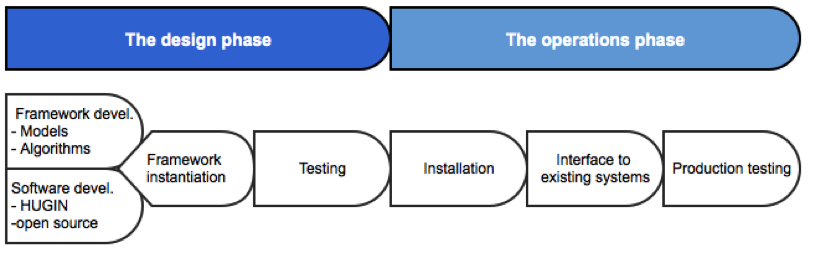
\includegraphics [keepaspectratio,width = 14cm] {REprocess2}
\caption{The table show key steps in the design and operation stages. Notice that each requirement can only be member of one step.} 
\label{REprocess2}
\end{figure}

The design stage contains general functionality requirements for the system, i.e. what the system should do and support.  In figure \ref{REprocess2}, we detail key steps inside this phase. The first step consists of the design of the general framework (models and algorithms) as well as the design and development of the software tools. In a second step, the general framework and software is instantiated for each specific use case. Finally, initial tests of the use case instantiated framework are conducted.  At the design phase, possible design requirements could e.g. address
\begin{itemize}
 \item the scope of the model
 \item the interpretability of the learned models
 \item the extent and type of domain knowledge that can be integrated into the models
 \item documentation
\end{itemize}

The requirements for the operation phase concern the functionality of the deployed system. In figure \ref{REprocess2}, we decompose this phase into three stages: installation, interface to existing systems, and production testing. The requirements for this phase could e.g. address
\begin{itemize}
 \item hardware constraints
 \item interfaces to existing software or data base systems
 \item inference functionality, i.e., what queries the system should be able to answer
\end{itemize}

\subsubsection*{Requirements and work packages allocation}

To make sure that all requirement comply with the document of work that is agreed upon upfront, every requirement is linked with the deliveries that are relevant.  This is clearly a tool to mitigate characteristic one.

\subsubsection*{Requirements prioritization}

In the Amidst RE process, the industrial partners are asked to categorize every requirement as an either must, should or could requirement.  Moreover, they are also asked to give rigorous prioritization of each requirement.  The intention is that the industrial partners are forced to think thoroughly about every requirement and how it relates to solving their problems.  This is a way to mitigate characteristic five.

\subsubsection*{The activities in the AMIDST requirements engineering process}
\label{sec:reprocess}

The activities in the requirement engineering process is carried out in an iterative fashion that is expected to involve a high level of cooperation and interaction between the partners in order to meet all characteristics in subsection \ref{sec:characteristics}. 

In figure \ref{REprocess1}, an illustration of the requirement engineering process for AMIDST is given, which is inspired by \cite{Ebe10}.  In general the process contain five phases, which are discussed below.
\begin{enumerate}
\item Preparation I.  This phase starts at the same time as work package one and ends when the initial template, attachment X1, for the requirement engineering document is finished.  In this template, the requirement engineering process is outlined including definitions of use cases, user groups and how to link requirements with stages in development process.  In order to meet characteristic three, four and five, the use case providers are asked to provide a detailed description of the system context that the AMIDST software is expected to run in, identify user groups, describe use cases and requirements.  In order to meet characteristic four, the requirements are linked with references to stages in the development cycle. 
\item Elicitation. The distribution of the above mentioned template marks the initialization of this phase.  Its aim is to get an initial high-level description of the different use cases and their requirements. This information are specified by the use case providers in collaboration with the academic partners to meet characteristic one, three and four.  Once the use case providers return the present document with the requested information, feedback and informal meetings are expected to clarify and refine the information provided.  At the end of the elicitation phase, the aim is to have a first coherent description of the requirements for each use case provider.
 \item Prioritization. In this phase the use case providers completes an extended version of the document template used in the previous phase. This template is used to link each of the requirements to the relevant work packages and tasks in the AMIDST project to meet characteristic one. Moreover, the template allows the use case providers to provide a more fine grained prioritization of the relevant requirements for the AMIDST framework.  Specifically, the use case providers are asked to rate each requirement in terms of must, should and could and also rate how important the requirement is to them.  
\item Validation. In this phase, the requirements from all use-case providers are collected to get the \emph{big picture}.  This involves a discussion to what extent the requirements can be accommodated. Revisions and negotiations of the detailed requirements are therefore expected.  In this phase, it is important to ensure that characteristic one is met.
 \item Evaluation and Testing. In this phase, the focus is on the elicitation of the evaluation and testing procedures in the AMIDST project. This phase starts with the distribution of a new document template, where the aim is to obtain a high level description of the evaluation and testing methods that is necessary to measure the performance of the AMIDST framework.
\end{enumerate}

\begin{figure}
\centering
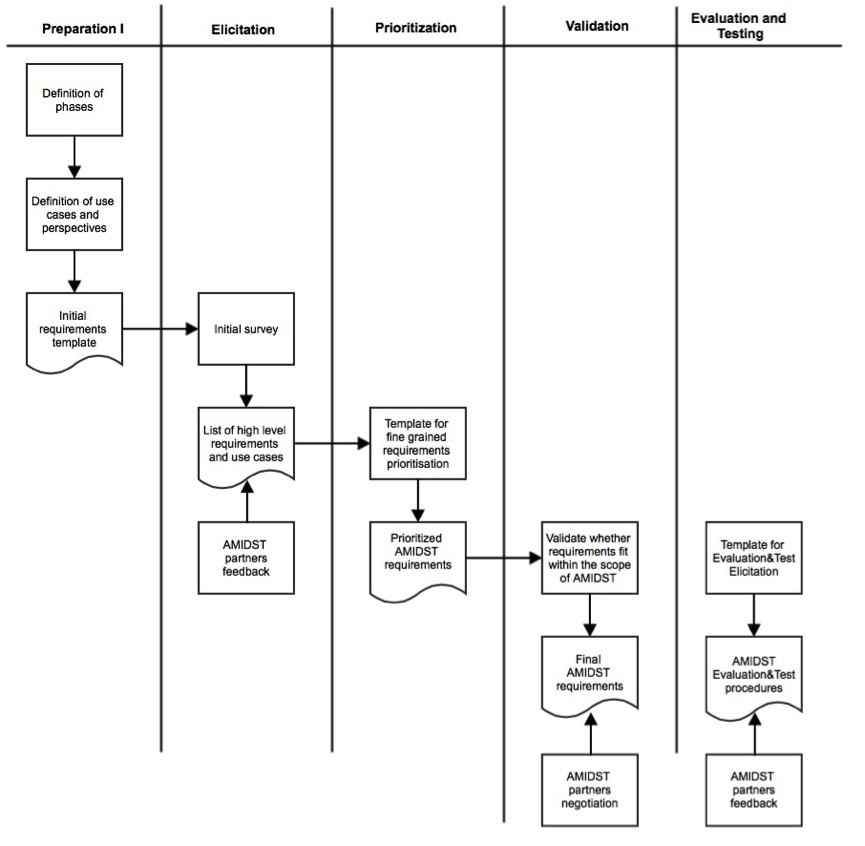
\includegraphics [keepaspectratio,width = 14cm] {REprocess1}
\caption{Description of the five phases in the requirement engineering process in AMIDST.}
\label{REprocess1}
\end{figure}
